\chapter{Interfacing With The Kinect Sensor}
\ifpdf
    \graphicspath{{Chapter3/Chapter3Figs/PNG/}{Chapter3/Chapter3Figs/PDF/}{Chapter3/Chapter3Figs/}}
\else
    \graphicspath{{Chapter3/Chapter3Figs/EPS/}{Chapter3/Chapter3Figs/}}
\fi

% ------------------------------------------------------------------------

The Kinect SDK provides access to the Kinect Sensor from within C\# code by defining a \verb|KinectSensor| object which interfaces directly with the hardware. When this object is instantiated, and provided a Kinect Sensor is connected via the USB port, it provides access to the depth, RGB and skeletal streams of the sensor. The \verb|KinectSensor| object also contains an event  \verb|AllFramesReady| which fires each time the streams have successfully updated. The streams update at approximately 30 frames per second but this rate can be significantly reduced if the sensor attempts to track too many skeletons.

Using this \verb|KinectSensor| object we built a general purpose skeletal tracking controller class \verb|GestureController| (Figure: ~\ref{fig:umlgest}) which initialises a \verb|KinectSensor| object to provide a single skeletal stream (for the left most person in the camera shot) and subscribes to the \verb|AllFramesReady| event via the method \verb|KinectAllFramesReady|. By extending this class we built two controllers for the two different modes of the SignAlign system. The first is used to record the positions of the joints for the skeleton for use as training data for the sign classifiers, the second is used to read a stream and use it along with our trained system to identify a sign.

\section{Recording Training Data}
In order to record the training data we implemented the classes \verb|GestureRecorder| and \verb|GestureRecording| (Figure: ~\ref{fig:umlgest}). This second class contains ten lists of 3-tuples of floats, one list for each joint tracked by the Kinect Sensor, and a method \verb|addReading| which takes a Skeleton object and adds each joint location to the appropriate list. The \verb|GestureRecorder| class stores a list of completed \verb|GestureRecording| objects along with one which is the current recording. This class extends \verb|GestureController| by implementing the \verb|KinectAllFramesReady| method to pass the Skeleton provided by the sensor to the \verb|currentRecording| object which stores the joint locations. This class also provides methods to start and stop the current recording (adding it to the list of recordings when stopped) and to save the list of recordings to file.


\begin{figure}[h!]
        \centering
        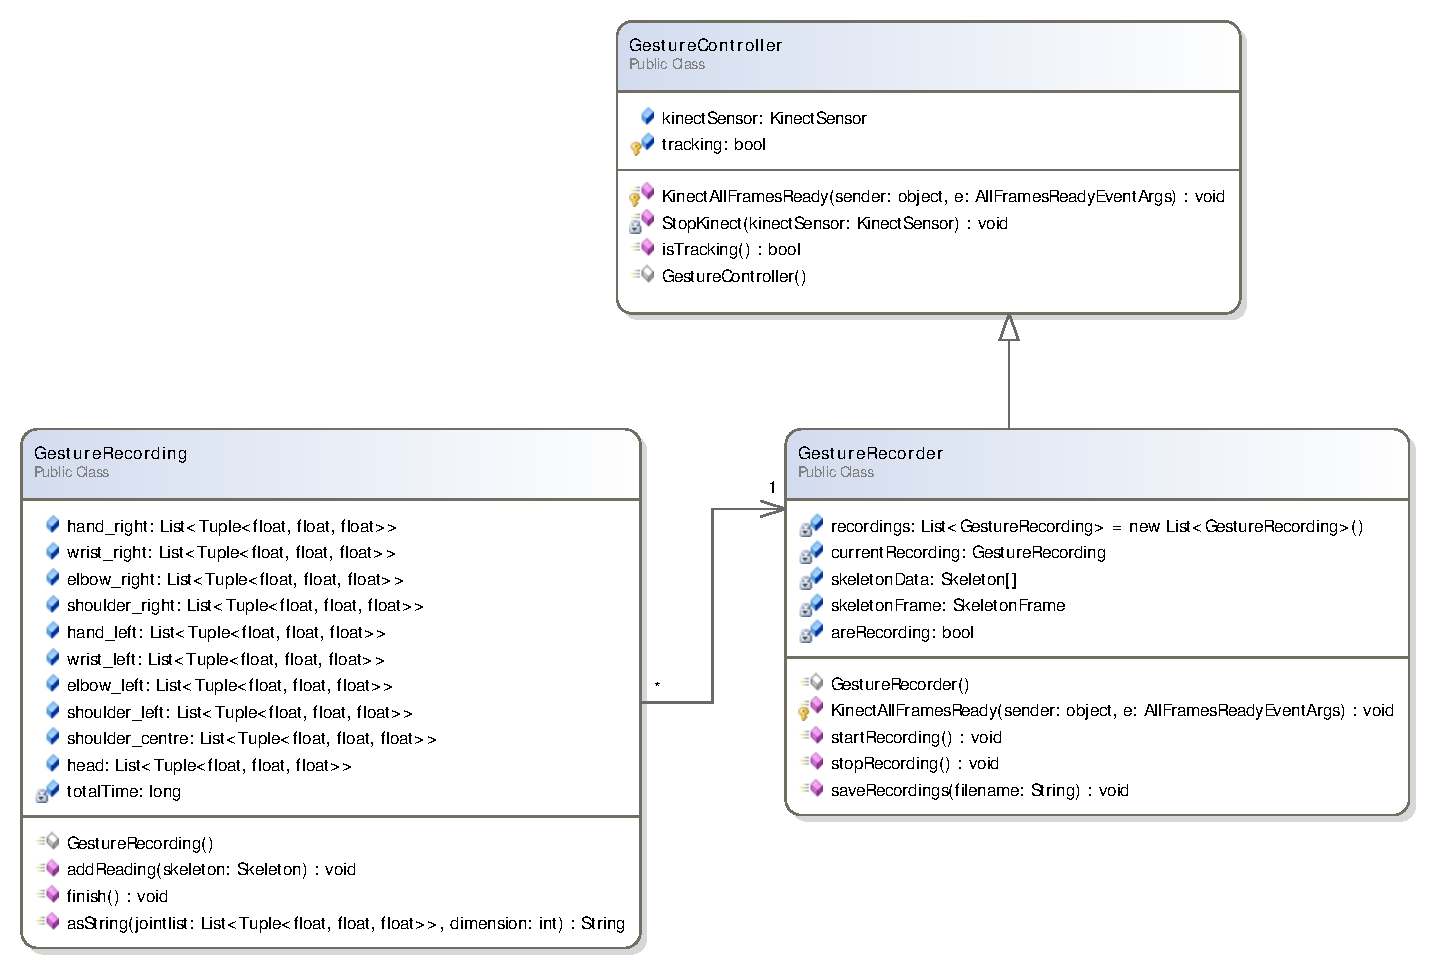
\includegraphics[width = 1.0\textwidth]{ThesisFigs/gestRecDiag}
        \caption{A UML diagram of the gesture recording classes}\label{fig:umlgest}
\end{figure}

Using this controller we implemented a small program which can be used to record a collection of training data by repeating sign the desire number of times and giving a start/stop signal between each. For convenience we defined this signal to be when the hand remains stationary for 2 seconds and is above the waist as this ensures that the signal is unlikely be given accidentally and will not corrupt the recording of the sign - as the hand can start at the beginning of the sign (and not at some arbitrary point).

\section{A Controller for Detecting Gestures}

 



%%% Local Variables: 
%%% mode: latex
%%% TeX-master: "../thesis"
%%% End: 
